\chapter{Detrending}\label{chap:detrending}

\section{Introduction}

Detrending is a signal processing technique aimed at removing long-term trends from data to isolate fluctuations that are more relevant for analysis. In the context of underwater acoustic target recognition, detrending can suppress broadband noise and highlight transient features, such as the periodic signals generated by ship machinery, which are critical for classification tasks. By removing these underlying trends, the remaining signal may provide cleaner, more interpretable inputs for machine learning models.

This chapter explores the application of $\ell_1$ detrending, a robust technique that builds on traditional methods like the Hodrick-Prescott filter. The goal of this experiment is to evaluate whether $\ell_1$ detrending can enhance the performance of the baseline CNN-LSTM model by improving the clarity of spectrogram features used for classification. Through this investigation, we seek to address a fundamental question: does detrending improve machine learning model performance in the field of underwater acoustics, or does it inadvertently remove essential features needed for accurate classification? 

\section{Overview of detrending algorithms}

Detrending algorithms aim to remove underlying trends from data, isolating the fluctuations that are more relevant for analysis. Mathematically, we can describe this as idea as an optimisation problem. We are given a scalar time series $y_t$, $t = 1, \ldots, n$, assumed to consist of an underlying slowly varying trend $x_t$, and a more rapidly varying random component $z_t$. Our goal is to estimate the trend component $x_t$, or equivalently, estimate the random component $z_t = y_t - x_t$. 

The simplest detrending method involves differencing the data. For a dataset with points $(x_1, x_2, \ldots, x_n)$, detrending by differencing computes a new dataset as $(x_2 - x_1, x_3 - x_2, \ldots, x_n - x_{n-1})$. While straightforward, this method can be overly sensitive to noise, as it does not distinguish between the trend and high-frequency fluctuations.

Another widely used approach is to detrend by fitting a model to the data and removing the fitted trend. A simple example is linear detrending, where a line is fit to the data via least squares regression, and the residuals make up the detrended result. More complex versions of this technique involve fitting higher-order polynomials or other parametric models to capture nonlinear trends.

One of these more sophisticated methods is the Hodrick-Prescott (H-P) filter, a technique popularised in the 1990s originally for use in economics \cite{hodrick_postwar_1997, whittaker_new_1922}. The H-P filter is widely used in time-series analysis to decompose a signal into its trend and cyclical components. It does so by solving an optimisation problem that minimises a loss function, balancing two competing objectives: fitting the trend closely to the data and ensuring the smoothness of the trend. Specifically, the H-P filter minimises:
\begin{equation}
    \sum_{t=1}^n (y_t - x_t)^2 + \lambda \sum_{t=2}^{n-1} (x_{t-1} - 2x_t + x_{t+1})^2
\end{equation}
where $y_t$ is the observed signal, $x_t$ is the trend, and $\lambda$ is the smoothing parameter. The first term enforces the trend's closeness to the original data, while the second term penalises sharp changes in the trend to ensure smoothness.

The smoothing parameter $\lambda$ plays a crucial role: larger $\lambda$ values result in smoother trends, while smaller $\lambda$ values retain more of the original signal's variability. While the H-P filter is effective for detecting long-term trends in economic data, it has limitations. It assumes that the trend is smooth, making it less effective for signals with sharp changes or localised features. Additionally, its reliance on the $\ell_2$ norm in the smoothness term can make it sensitive to outliers which can disproportionately affect the squared differences.

\subsection{\texorpdfstring{$\ell_1$}{l1} Detrending Algorithm}
The $\ell_1$ detrending algorithm \cite{kim_ell_1_2009} builds on the principles of the H-P filter but replaces the $\ell_2$ norm in the smoothness penalty with the $\ell_1$ norm. This modification makes the $\ell_1$ algorithm more robust to outliers and better suited to capturing sharp changes in the trend. The optimisation problem for $\ell_1$ detrending is expressed as:
\begin{equation}
    \frac{1}{2} \sum_{t=1}^n (y_t - x_t)^2 + \lambda \sum_{t=2}^{n-1} \| x_{t-1} - 2x_t + x_{t+1} \|
\end{equation}
Here, the $\ell_1$ norm ($\| \cdot \|$) in the second term penalises large differences between successive points in the trend, enforcing smoothness while preserving sharp transitions.

The $\ell_1$ detrending algorithm retains the flexibility of the H-P filter with its tunable regularisation parameter $\lambda$, but its use of the $\ell_1$ norm allows it to better handle datasets with localised events or abrupt changes. Ship radiated noise, for instance, often contains periodic narrowband features from machinery noise, which can be masked by the broadband components in the signal. The $\ell_1$ algorithm’s sensitivity to these features makes it particularly suitable for UATR tasks. By fine-tuning $\lambda$, we can strike a balance between removing the trend and preserving the narrowband features critical classification.

\section{Experiments}

To evaluate the impact of detrending on underwater acoustic target recognition, we designed an experiment to assess the performance of our benchmark CNN-LSTM model with spectrograms processed under varying levels of $\ell_1$ detrending. By removing long-term trends and broadband noise from the spectrograms, the objective of this experiment is to determine whether detrending enhances classification accuracy by isolating meaningful features while suppressing irrelevant signal components. 

\subsection{Methodology}

The $\ell_1$ detrending algorithm was implemented in MATLAB as a modular and flexible function which builds upon the original code published by the authors. The primary objective of this implementation was to enable experimentation with different detrending strengths through tweaking the regularisation parameter $\lambda$, to which we assign a coefficient $\alpha$, as well as provide visualisations to evaluate the effectiveness of detrending for classification and image segmentation tasks.

Recall that the detrending algorithm is formulated as an optimisation problem where we try to balance two objectives: minimising the residual between the input signal and its estimated trend while ensuring that the trend remains smooth. The regularisation parameter $\lambda$ governs this trade-off. For any given signal, $\lambda_{\text{max}}$ is the value of $\lambda$ beyond which the algorithm will simply return a 1-to-1 translation, or \textit{affine fit}, for the data. This upper bound is computed using a function provided by the authors, \texttt{l1tf\_lambdamax}. The value of $\lambda$ used during detrending is then defined as a fraction of $\lambda_{\text{max}}$, controlled by our assigned coefficient $\alpha$. By experimenting with various values of $\alpha$, it is possible to fine-tune the balance between trend smoothness and residual suppression.

\begin{figure}[htbp]
    \centering
    % Subfigure 1: Segment trend plot
    \begin{subfigure}[t]{\textwidth}
        \centering
        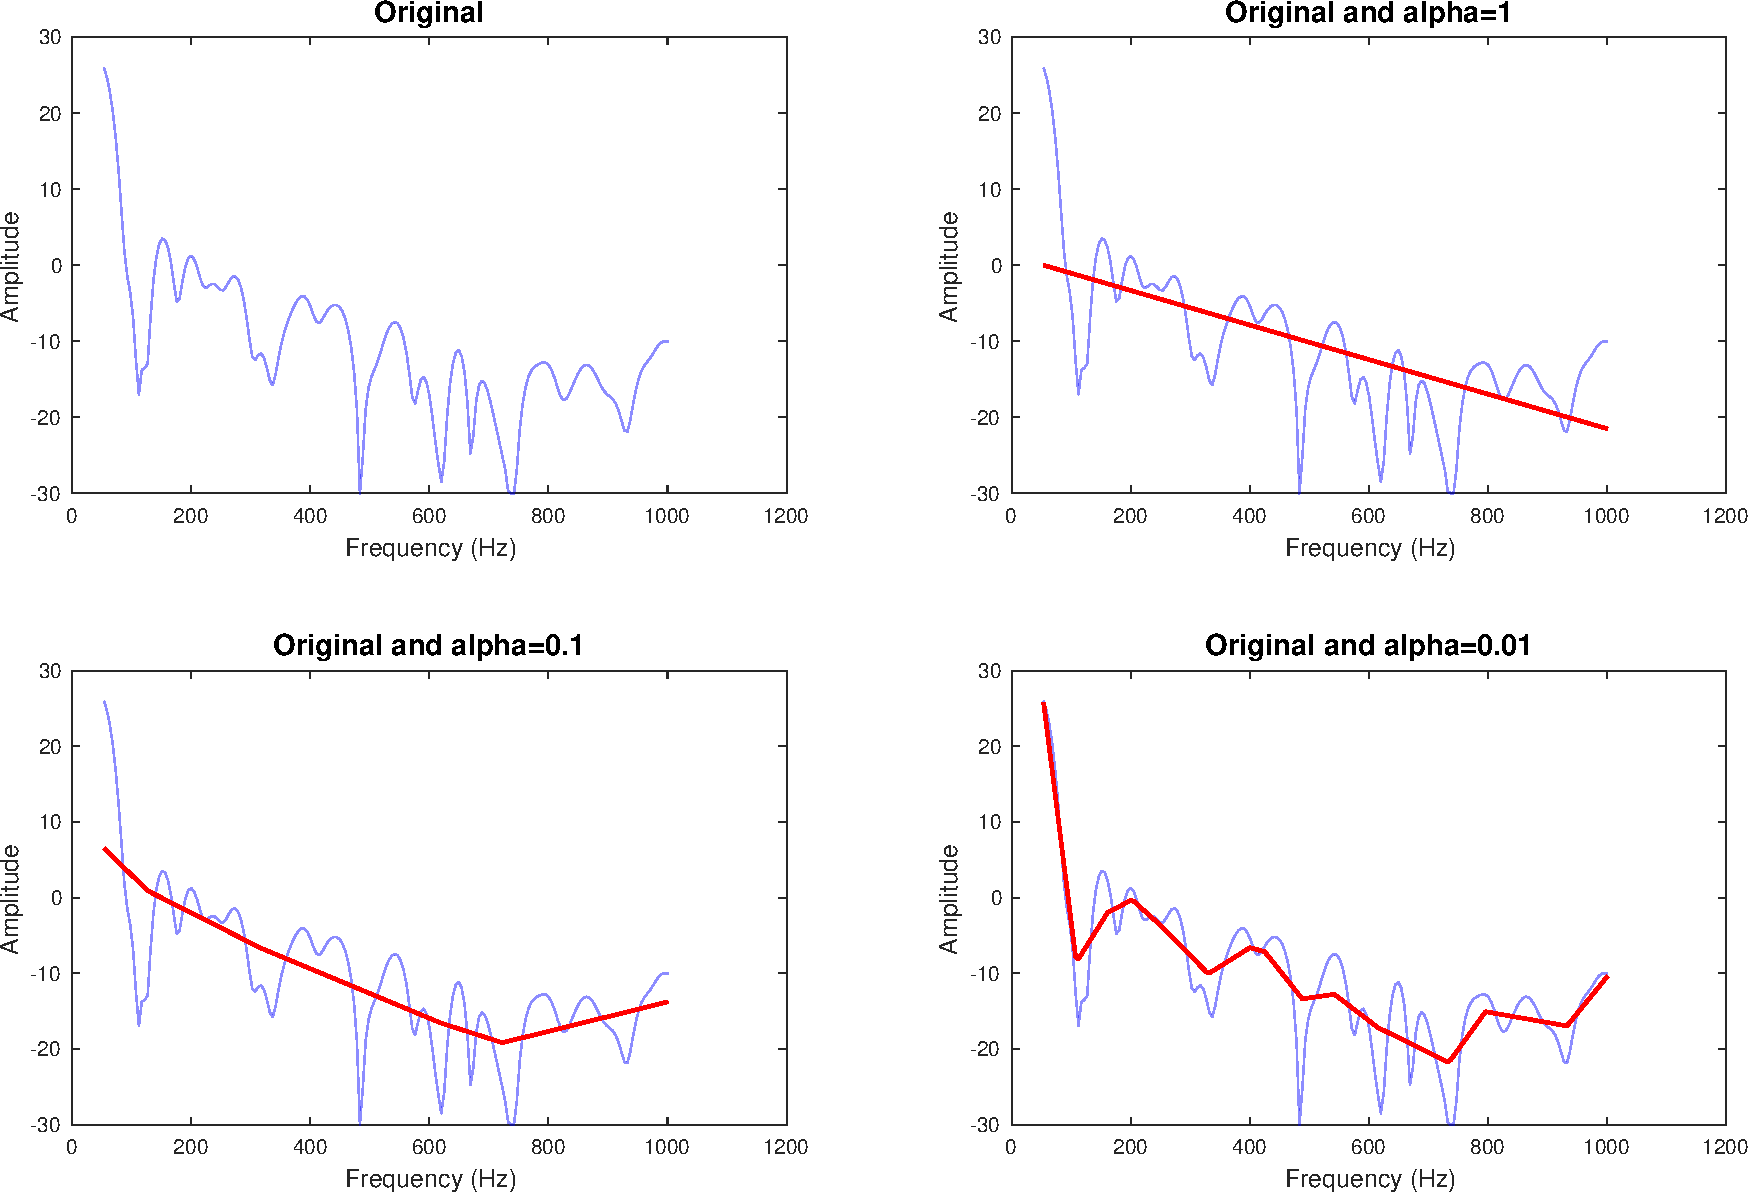
\includegraphics[width=0.95\textwidth]{img/ch5/example_l1_plots/segment_l1_trend.pdf}
        \caption{Overlay of a random time segment with its corresponding $\ell_1$ trend at various $\alpha$ values.}
        \label{fig:l1:segment-trend}
    \end{subfigure}
    
    \vspace{1cm}
    
    % Subfigure 2: Segment detrended plot
    \begin{subfigure}[t]{\textwidth}
        \centering
        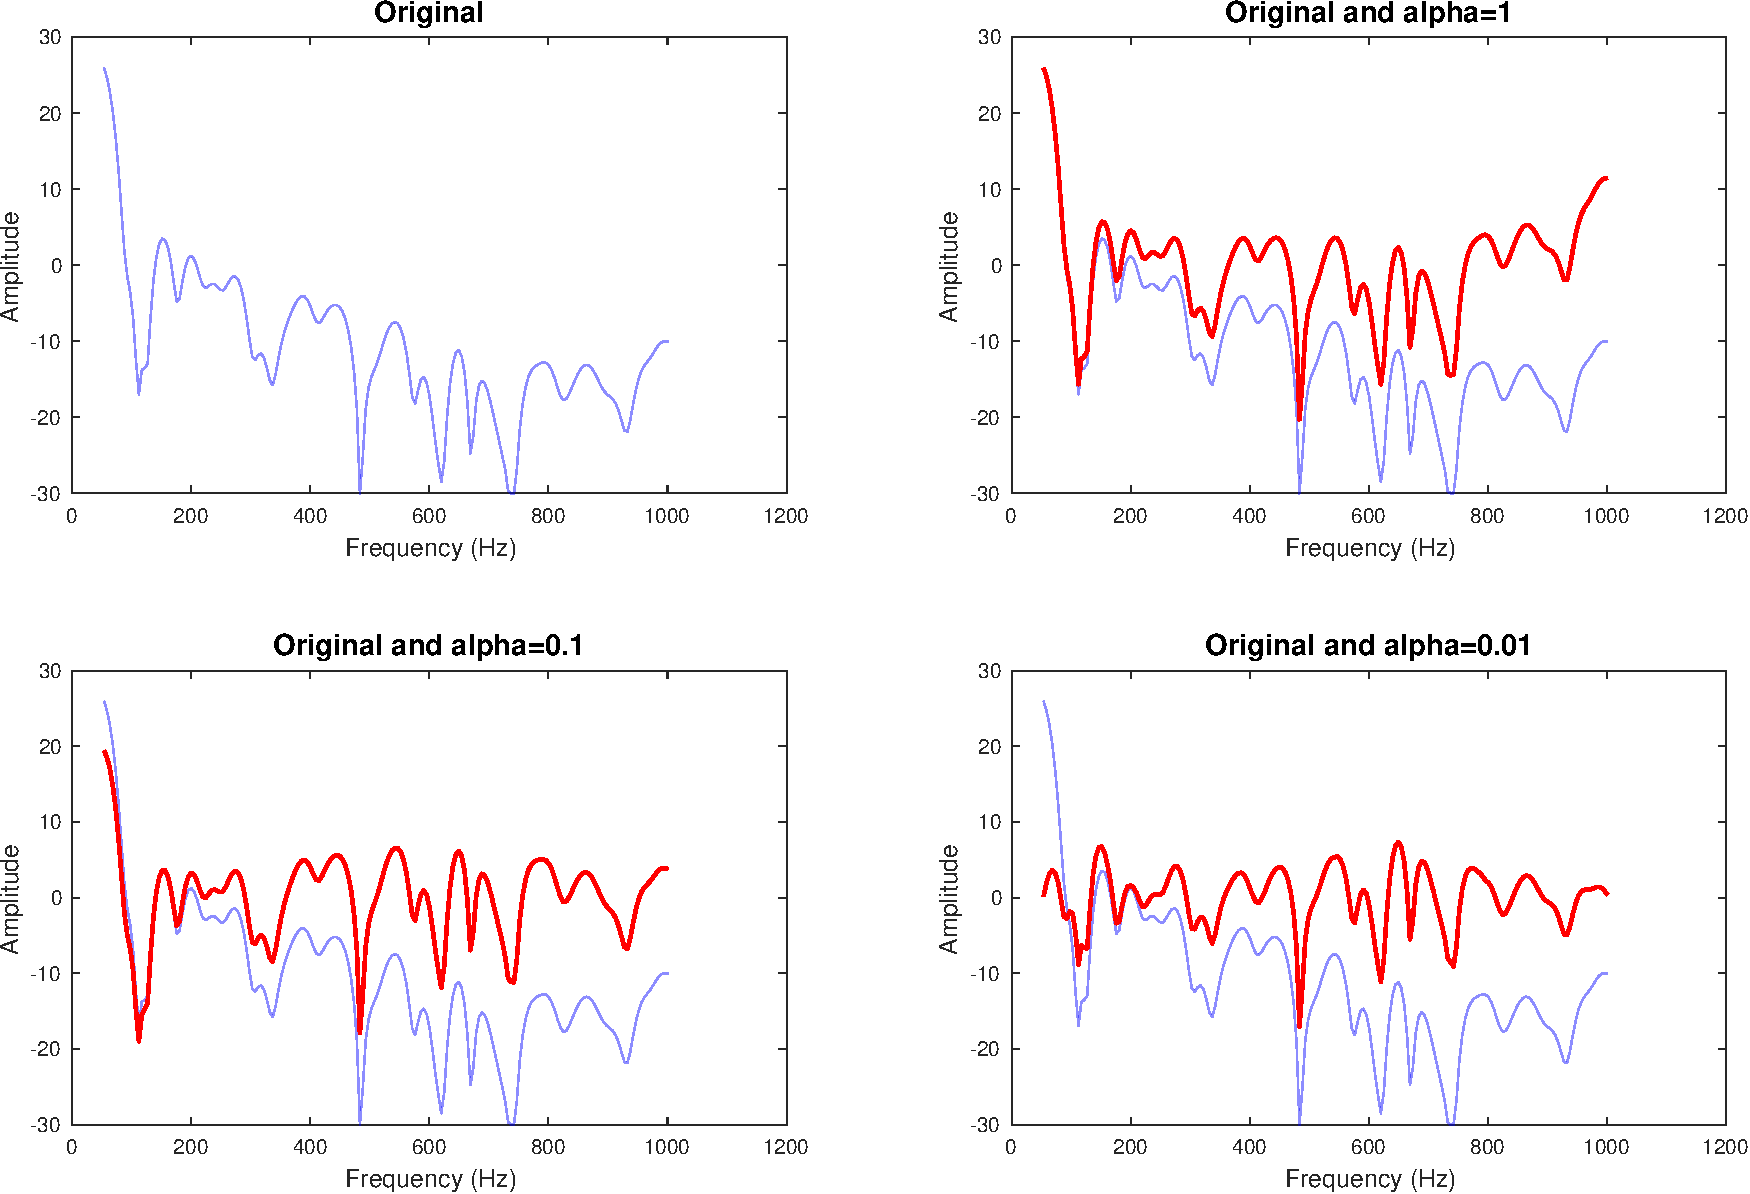
\includegraphics[width=0.95\textwidth]{img/ch5/example_l1_plots/segment_detrended.pdf}
        \caption{Random time segment before and after detrending at different $\alpha$ values, highlighting the removal of long-term trends in the signal.}
        \label{fig:l1:segment-detrended}
    \end{subfigure}
\end{figure}

\begin{figure}
    \ContinuedFloat
    % Subfigure 3: Spectrogram comparison
    \begin{subfigure}[t]{\textwidth}
        \centering
        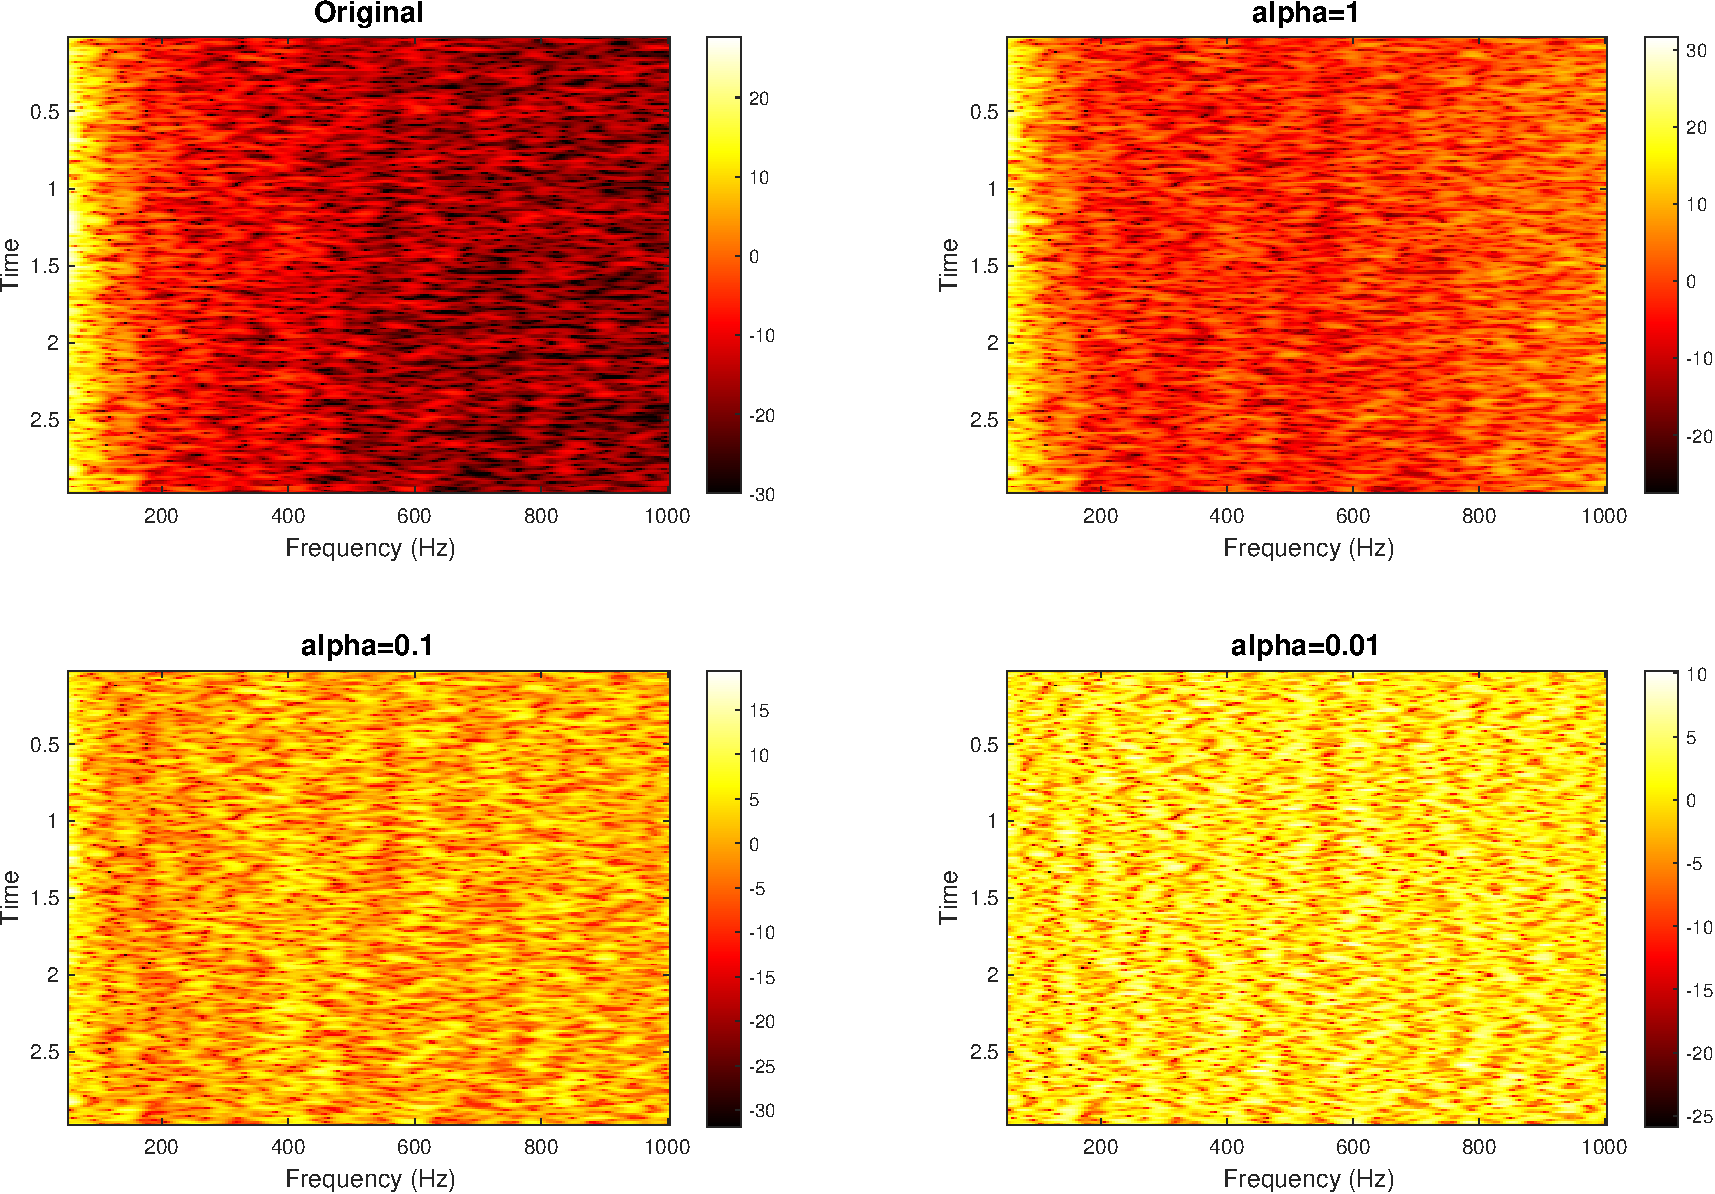
\includegraphics[width=0.92\textwidth]{img/ch5/example_l1_plots/spec_comparison.pdf}
        \caption{Comparison of original and detrended spectrograms produced using $\ell_1$ detrending at various $\alpha$ values.}
        \label{fig:l1:spectrogram-comparison}
    \end{subfigure}
    
    \vspace{1cm}
    
    % Subfigure 4: 3D surface plots
    \begin{subfigure}[t]{\textwidth}
        \centering
        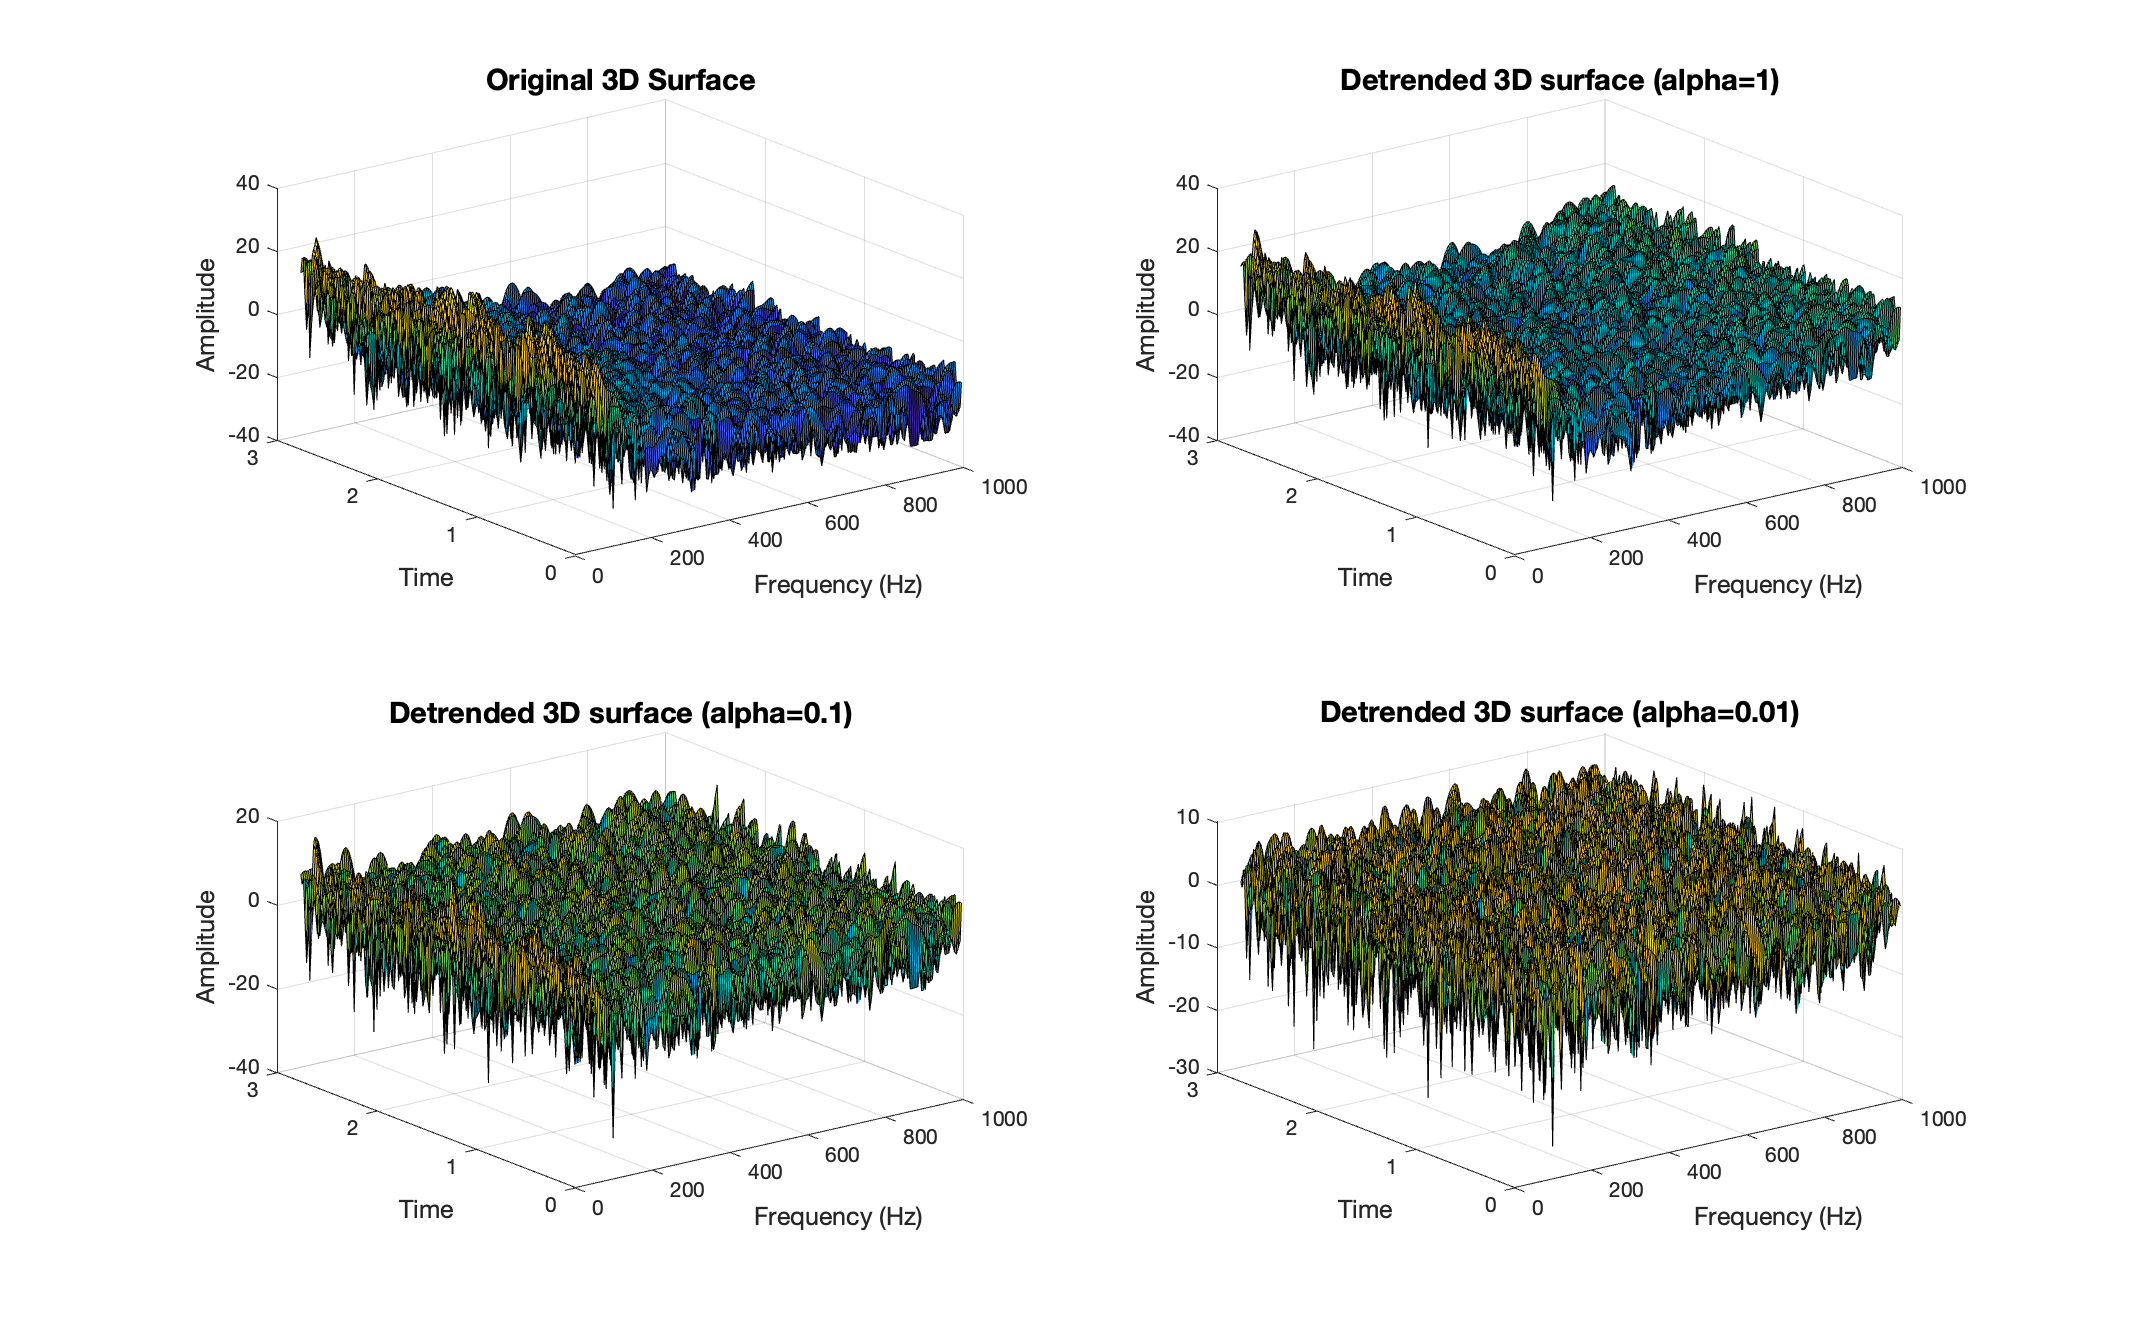
\includegraphics[trim={3cm 1.5cm 2.5cm 1cm},clip,width=0.92\textwidth]{img/ch5/example_l1_plots/3d_plot.pdf} %{left bottom right top}
        \caption{Three-dimensional surface plots of the original spectrogram and detrended spectrograms at different $\alpha$ values.}
        \label{fig:l1:3d}
    \end{subfigure}
    \caption{Visual analysis of $\ell_1$ detrending for various $\alpha$ values, illustrating its impact on spectrograms through comparative visualisations, time-segment overlays, and 3D surface plots.}
    \label{fig:l1:overview}
\end{figure}

To support this experimentation, our implementation of the $\ell_1$ detrending algorithm allows the user to specify up to 10 values of $\alpha$ in a single run. The function computes detrended spectrograms for each specified $\alpha$ value and generates a range of diagnostic plots that facilitate analysis. 
\begin{enumerate}
    \item Segment trend plot: This plot (Figure~\ref{fig:l1:segment-trend}) overlays a single random time segment with its corresponding $\ell_1$ trends for various $\alpha$ values. 
    \item Segment detrended plot: This diagnostic (Figure~\ref{fig:l1:segment-detrended}) shows the same time segment before and after detrending for various $\alpha$ values. It is the most helpful diagnostic plot to visualise the changes introduced by detrending, especially the removal of long-term trends such as those created by background noise. By examining the degree of smoothing introduced for different $\alpha$, we could evaluate how effectively the algorithm removed noise without discarding important signal features. Smaller $\alpha$ values were observed to retain more signal detail but were less effective at suppressing noise, while larger $\alpha$ values removed noise more aggressively but often smoothed out transient features.
    \item Spectrogram comparison: This diagnostic plot (Figure~\ref{fig:l1:spectrogram-comparison}) presents the original spectrogram alongside detrended spectrograms generated using different $\alpha$ values. It provides an overview of how detrending affects the overall amplitude structure, particularly in regions dominated by long-term trends or broadband noise. By visually assessing these plots, we could identify the boundaries where detrending was either too aggressive (overfitting) or too weak (underfitting).
    \item 3D surface plots: These 3D plots (Figure \ref{fig:l1:3d}) provide an alternative representation of how detrending impacts amplitude values across time and frequency.
\end{enumerate}

Using these diagnostic plots, we determined that $\alpha$ values in the range $[10^{-3}, 1]$ provided a suitable balance between noise suppression and signal preservation. Hence, we chose three such $\alpha$ values for further experimentation: $10^{-2}$, $10^{-1},$ and $1$. These values were chosen in hopes of capturing a wide spectrum of detrending strengths, ranging from subtle noise suppression to more aggressive trend removal.

Then, to evaluate the effect of $\ell_1$ detrending on UATR classification performance, the baseline 3-second DeepShip spectrograms (Section \ref{sec:inputs}) were processed using the three selected $\alpha$ values ($10^{-2}$, $10^{-1},$ and $1$). Each detrended spectrogram was saved to a separate directory as a \texttt{.mat} file and subsequently used as input to the CNN-LSTM baseline model.

The CNN-LSTM model was trained under identical conditions to the baseline model to ensure fair comparisons. The same architecture, hyperparameters, and training configuration were used for all experiments, as detailed in Table~\ref{tab:cnn-lstm-final-params} and Section~\ref{subsec:training-configuration}, and the same 10-fold cross-validation splits used in previous experiments were applied to ensure consistency and comparability across results.  Model performance was evaluated using accuracy as the primary metric, and training and validation loss curves were recorded to analyse convergence trends qualitatively.

To further ensure robustness, all experiments were conducted using MATLAB version 2024a and Keras 2.10, with a seeded random number generator and GPU-accelerated training. This setup, consistent with the baseline model, guarantees that any observed differences in model performance can be attributed solely to the effect of $\ell_1$ detrending and its parameter variations.

\subsection{Results}

The classification results for the $\ell_1$ detrending experiments, presented in Table \ref{tab:detrend-results-3s}, show that all three detrending configurations resulted in lower classification accuracy and precision compared to the baseline. The baseline model achieved an accuracy of 63.41\% and a precision of 66.53\%, whereas the detrended models showed a consistent decline, with accuracy reductions ranging from 15.19\% at $\alpha = 10^{-2}$ to 7.78\% at $\alpha = 0.1$. Precision followed a similar trend, with decreases across all $\alpha$ values. Training and validation accuracy-loss curves are shown in Figure \ref{fig:detrend-acc-loss-curves-epoch} and \ref{fig:detrend-acc-loss-curves-fold}.

\begin{table}[htbp]
    \centering
    \caption{Classification results using $\ell_1$ detrending algorithm at various $\alpha$.}
    \label{tab:detrend-results-3s}
    \begin{tabular}{lcc}
        \toprule
        \textbf{Detrending parameter} & \textbf{Accuracy (\%)} & \textbf{Precision (\%)} \\ \midrule
        $\alpha = 10^{-2}$            & 48.22 & 59.09 \\
        $\alpha = 10^{-1}$            & 52.03 & 62.54 \\
        $\alpha = 1$                  & 55.63 & 63.97 \\
        \textbf{Baseline (no detrending)}  & \textbf{63.41} & \textbf{66.53} \\
        \bottomrule
    \end{tabular}
\end{table}

\subsection{Discussion}

The consistent drop in accuracy across all $\alpha$ values suggests that $\ell_1$ detrending, while effective at removing long-term trends, may also be inadvertently removing or distorting features essential for classification.

Lower $\alpha$ values may be causing \textit{over-smoothing}; that is, the $\ell_1$ algorithm could be aggressively suppressing broadband noise through the removal of the long-term trend, but also smoothing out transient narrowband features such as machinery noise which are key discriminators for different vessel types. On the other hand, higher $\alpha$ values may be preserving finer details while failing to adequately suppress broadband noise: a phenomenon called \textit{under-suppression}. 

It is also possible that the short 3 second duration of the input segments (Section \ref{subsec:segmentation}) is preventing the $\ell_1$ algorithm from accurately capturing the broader trend of each recording. This could lead to incomplete or imprecise detrending.

\begin{figure}[p]
    \centering
    \begin{subfigure}{\textwidth}
        \centering
        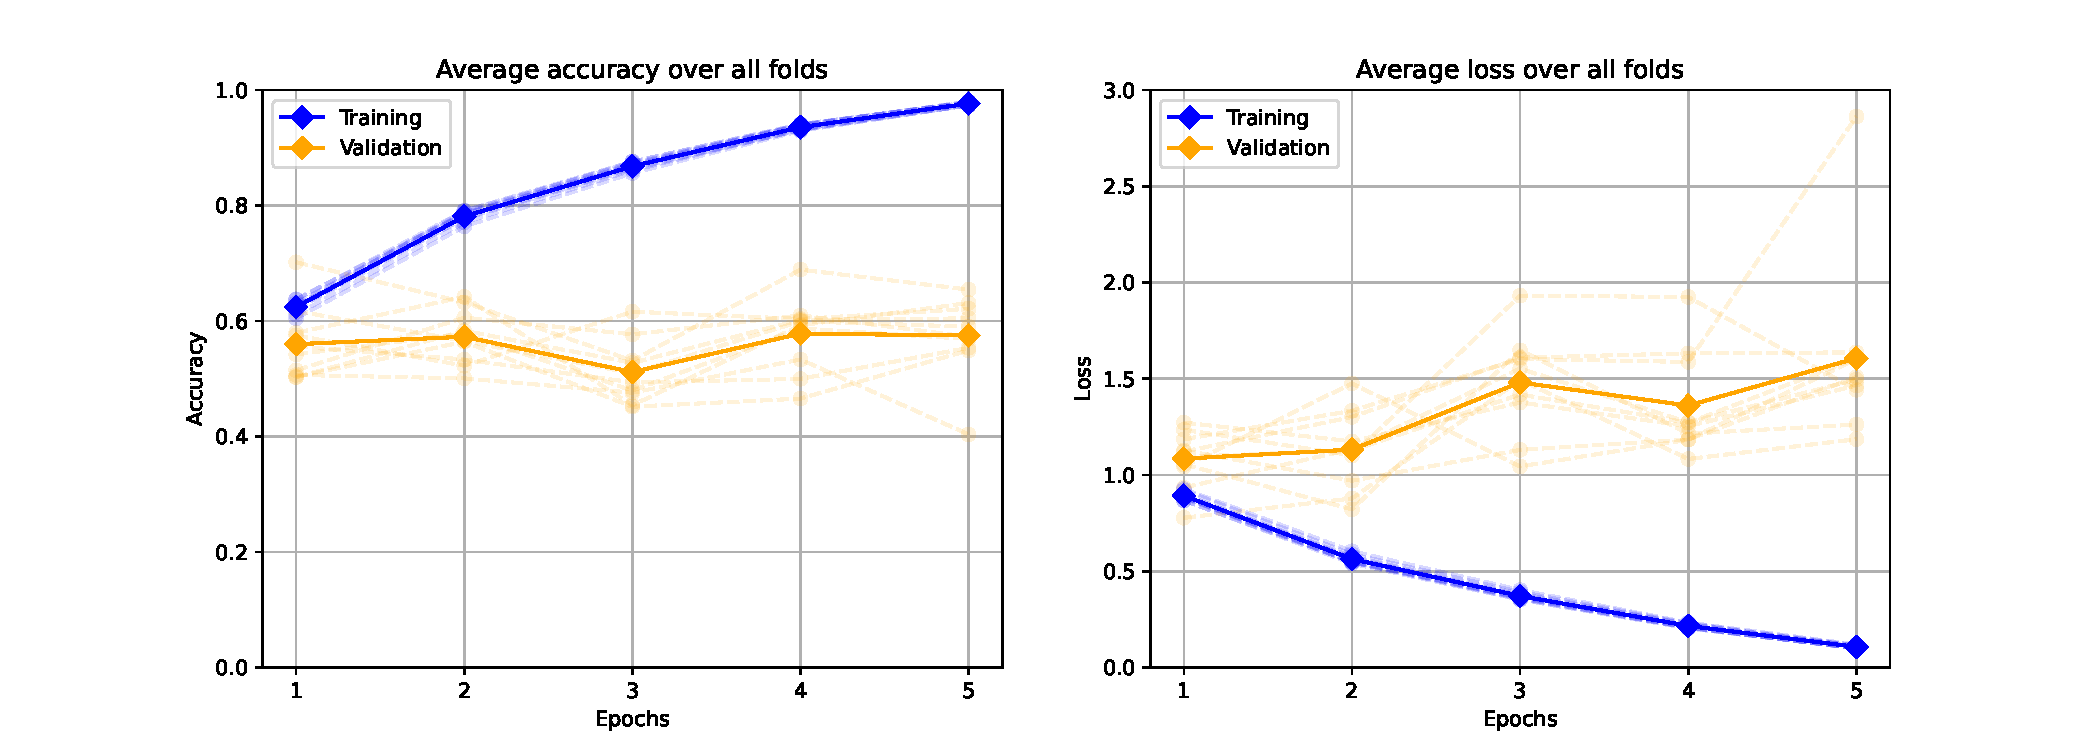
\includegraphics[trim={3cm 0 3cm 0.8cm},clip,width=\textwidth]{img/ch5/e0_3_epochs_by_epoch.pdf}
        \caption{Validation accuracy and loss by epoch for $\ell_1$ detrending with $\alpha = 1$.}
        \label{fig:detrend-acc-loss-e0-epoch}
    \end{subfigure}

    \vspace{0.5cm}
    
    \begin{subfigure}{\textwidth}
        \centering
        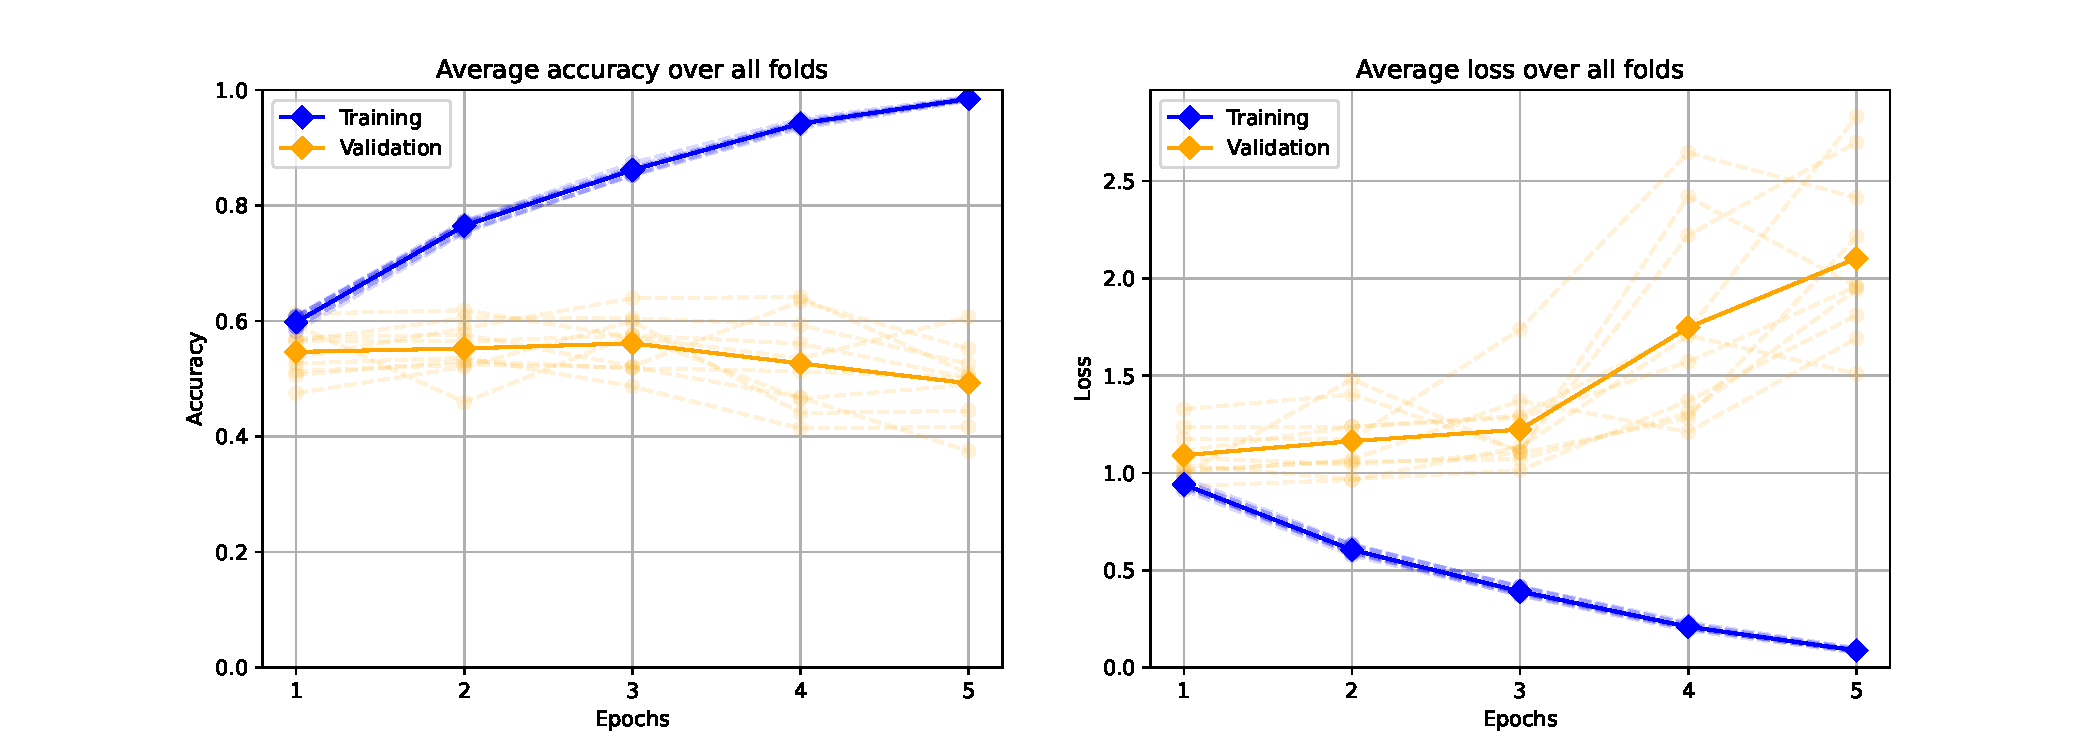
\includegraphics[trim={3cm 0 3cm 0.8cm},clip,width=\textwidth]{img/ch5/e-1_3_epochs_by_epoch.pdf}
        \caption{Validation accuracy and loss by epoch for $\ell_1$ detrending with $\alpha = 10^{-1}$.}
        \label{fig:detrend-acc-loss-e-1-epoch}
    \end{subfigure}

    \vspace{0.5cm}
    
    \begin{subfigure}{\textwidth}
        \centering
        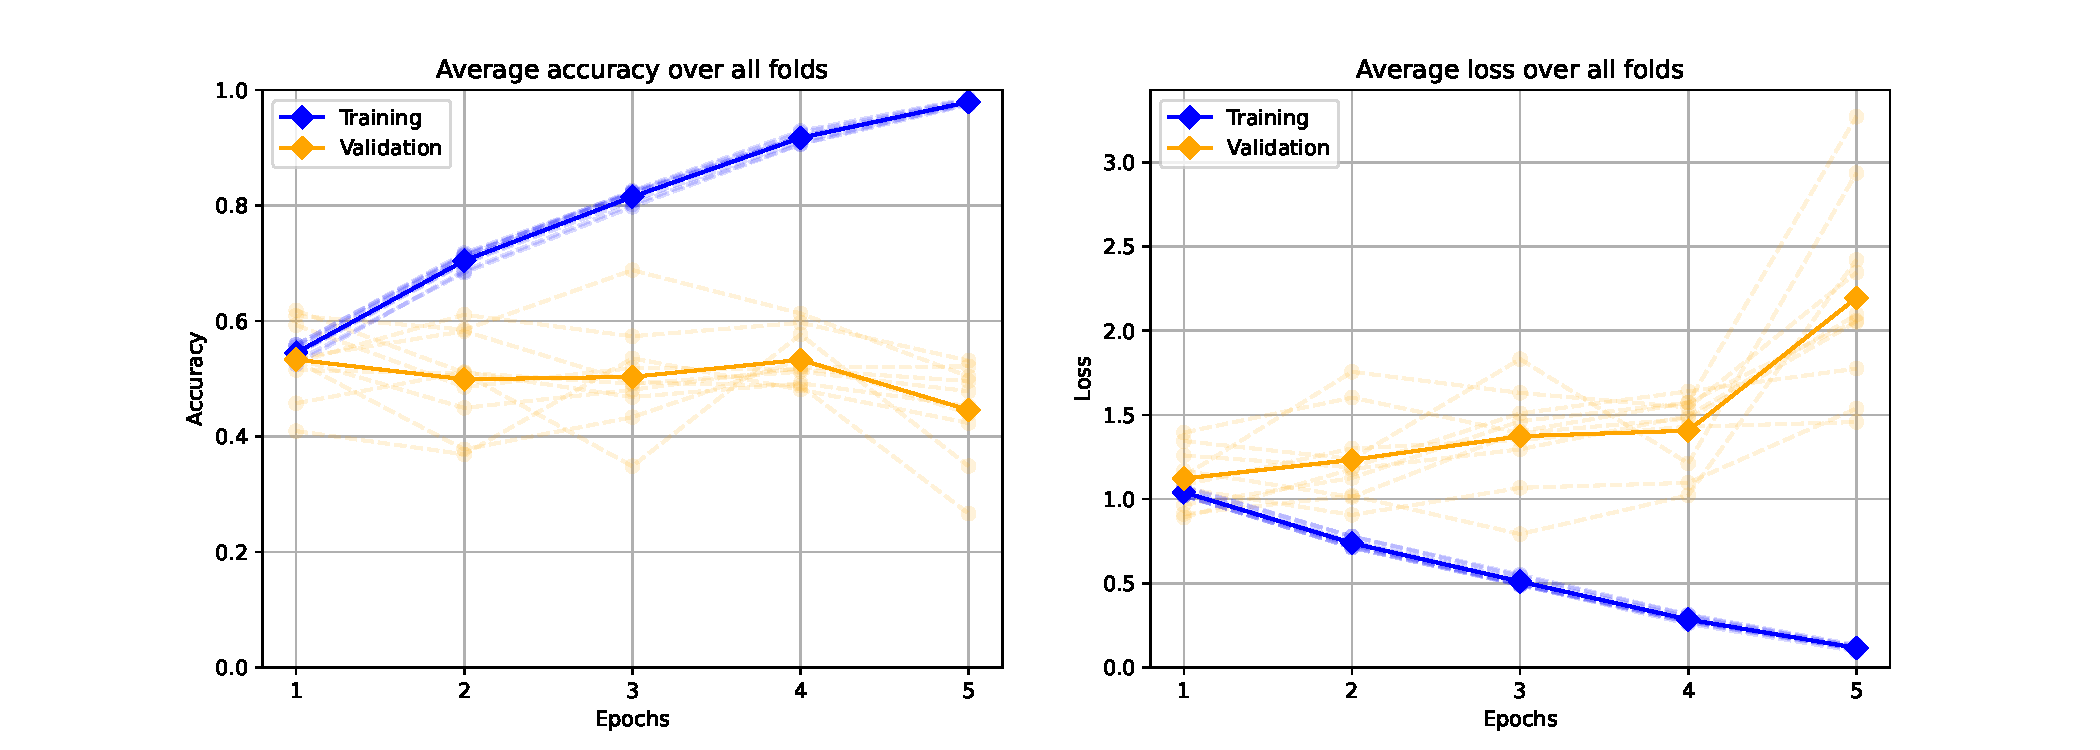
\includegraphics[trim={3cm 0 3cm 0.8cm},clip,width=\textwidth]{img/ch5/e-2_3_epochs_by_epoch.pdf}
        \caption{Validation accuracy and loss by epoch for $\ell_1$ detrending with $\alpha = 10^{-2}$.}
        \label{fig:detrend-acc-loss-e-2-epoch}
    \end{subfigure}
    \caption{Validation accuracy and loss curves for $\ell_1$ detrending experiments by epoch. Faint lines show curves for individual folds while the dark line shows the average across all folds.} 
    \label{fig:detrend-acc-loss-curves-epoch}
\end{figure}

\begin{figure}[p]
    \centering
    \begin{subfigure}{\textwidth}
        \centering
        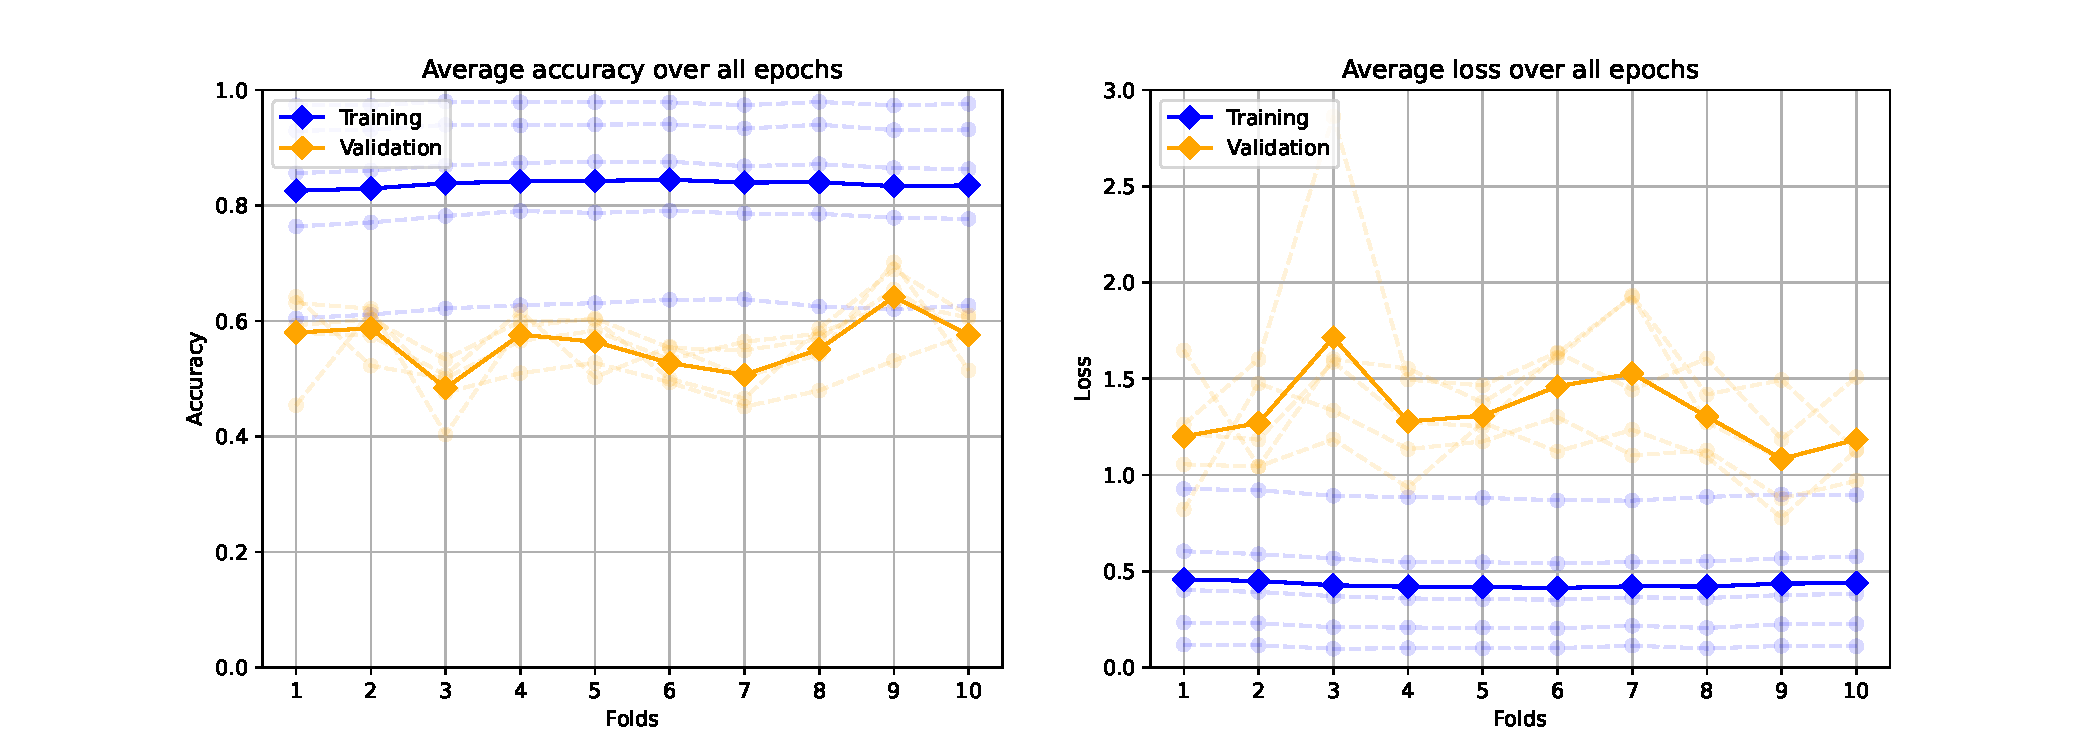
\includegraphics[trim={3cm 0 3cm 0.8cm},clip,width=\textwidth]{img/ch5/e0_3_epochs_by_fold.pdf}
        \caption{Validation accuracy and loss by fold for $\ell_1$ detrending with $\alpha = 1$.}
        \label{fig:detrend-acc-loss-e0-fold}
    \end{subfigure}

    \vspace{0.5cm}
    
    \begin{subfigure}{\textwidth}
        \centering
        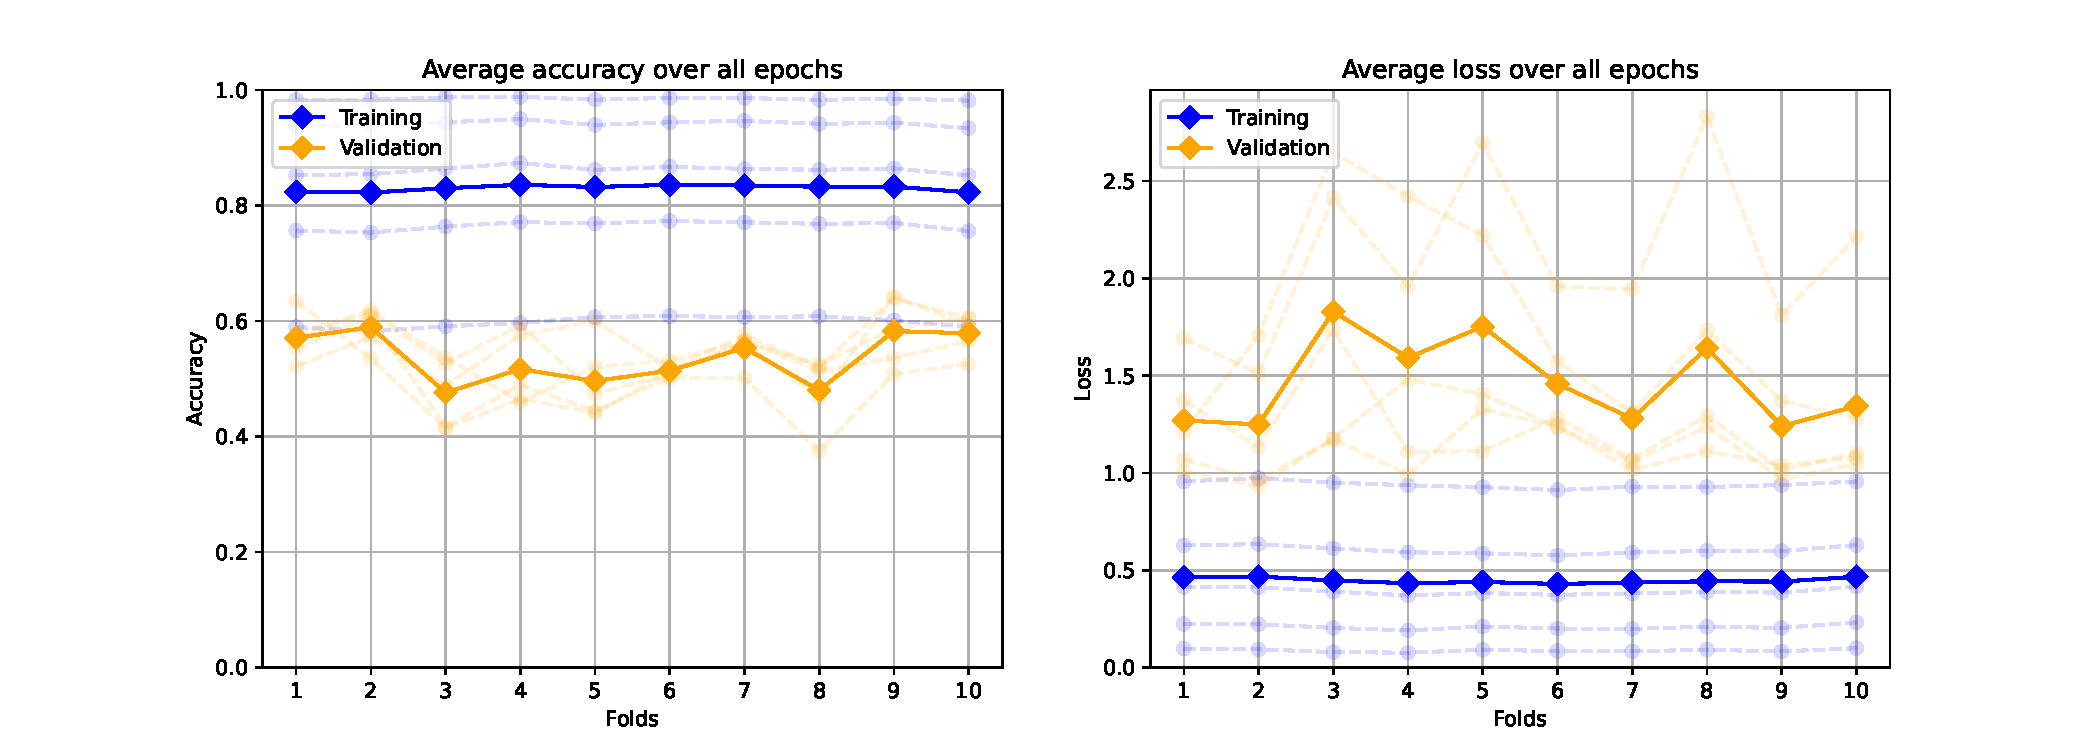
\includegraphics[trim={3cm 0 3cm 0.8cm},clip,width=\textwidth]{img/ch5/e-1_3_epochs_by_fold.pdf}
        \caption{Validation accuracy and loss by fold for $\ell_1$ detrending with $\alpha = 10^{-1}$.}
        \label{fig:detrend-acc-loss-e-1-fold}
    \end{subfigure}

    \vspace{0.5cm}
    
    \begin{subfigure}{\textwidth}
        \centering
        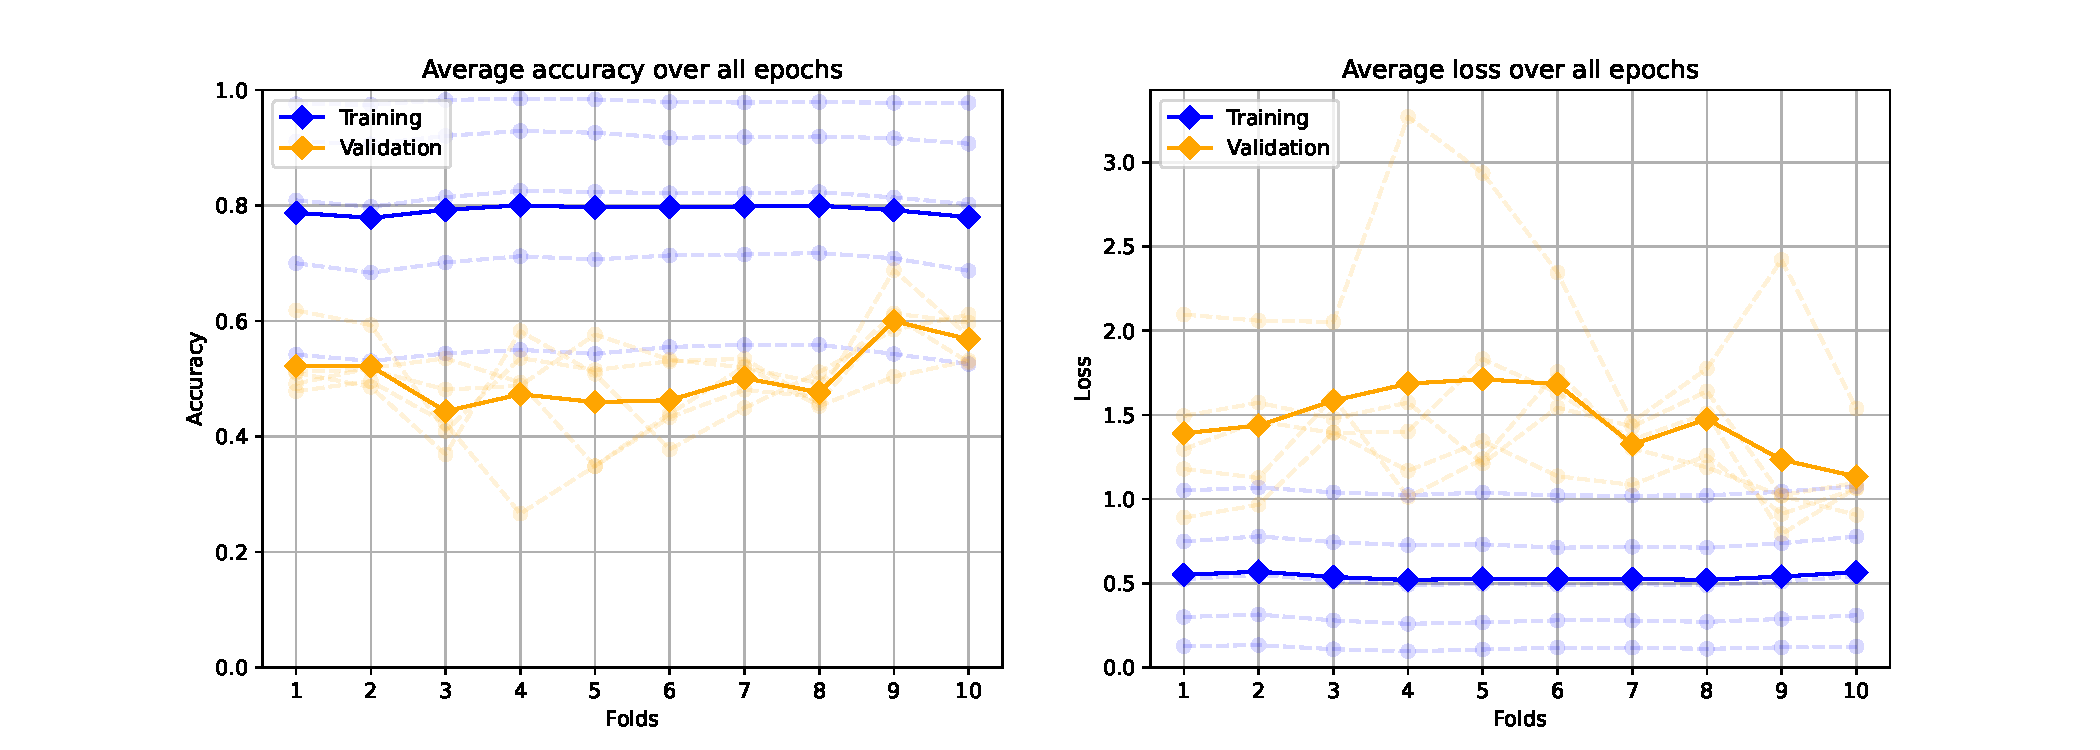
\includegraphics[trim={3cm 0 3cm 0.8cm},clip,width=\textwidth]{img/ch5/e-2_3_epochs_by_fold.pdf}
        \caption{Validation accuracy and loss by fold for $\ell_1$ detrending with $\alpha = 10^{-2}$.}
        \label{fig:detrend-acc-loss-e-2-fold}
    \end{subfigure}
    \caption{Validation accuracy and loss curves for $\ell_1$ detrending experiments by fold. Faint lines show curves for individual epochs while the dark line shows the average across all epochs.} 
    \label{fig:detrend-acc-loss-curves-fold}
\end{figure}

The poor results may further stem from the combined effect of using a detrending algorithm, which alters the spatial and temporal characteristics of the data, in tandem with a CNN-LSTM classifier, which heavily relies on these characteristics to perform classification (in fact, this was the primary reason for choosing this model; see Section \ref{sec:cnn-lstm-overview}). The $\ell_1$ algorithm may have disrupted the input, which is reflected in the instability of the accuracy-loss curves for the detrending experiments (Figures \ref{fig:detrend-acc-loss-curves-epoch} and \ref{fig:detrend-acc-loss-curves-fold}). In contrast to the uniform curves obtained for the baseline model (described in Section \ref{sec:baseline-results}), the accuracy-loss curves for the detrending experiments reveal significant irregularities. In Figure \ref{fig:detrend-acc-loss-curves-epoch}, the validation curves for individual folds deviate notably from the average trend, with erratic fluctuations that suggest inconsistent convergence. This issue is even more pronounced in Figure \ref{fig:detrend-acc-loss-e-1-fold}, where the validation loss curves for each epoch show dramatic variability. Such behaviour is indicative of challenges in the model's ability to learn and generalise effectively, suggesting that the DeepShop spectrograms may have lost important information in the detrending process which the CNN-LSTM model relied on for accurate classification. As a result, the model likely struggled to interpret the input features in a coherent way, leading to unstable performance and poor generalisation across folds.

Fundamentally, these findings raise questions about the appropriateness of detrending for \acrshort{uatr} tasks. While detrending is commonly used in domains like finance or EEG analysis, where trends often obscure the signal of interest, it may simply be that through removing long-term trends, the detrended spectrograms are losing the distinct structure necessary for the baseline CNN-LSTM model to effectively discern between vessel types.  

\subsection{Conclusion}

While $\ell_1$ detrending holds theoretical promise for its ability to suppress long-term trends, its practical application to \acrshort{uatr} tasks presents significant challenges. The classification performance of our baseline CNN-LSTM model declined when using $\ell_1$-detrended spectrograms across all tested $\alpha$ values, with accuracy and precision reductions suggesting the unintended removal or distortion of essential spectrogram features. Lower $\alpha$ values appeared to over-smooth transient features critical for vessel classification, while higher $\alpha$ values failed to adequately suppress broadband noise. Furthermore, the erratic accuracy-loss curves observed during training suggest that the detrending process disrupted the spatial and temporal structure of the spectrograms, hindering the CNN-LSTM model's ability to converge effectively.

Future work should investigate these effects more thoroughly. First, further investigation into the interaction between detrending and the CNN-LSTM architecture is needed to better understand the underlying causes of the poorly-behaved accuracy and loss training curves. It may also be valuable to explore the effects of detrending on other model architectures to assess whether the observed issues are specific to the CNN-LSTM framework. Additionally, experimenting with a wider range of $\alpha$ values could help identify configurations that strike a better balance between noise suppression and the preservation of key features. Extending the length of the input audio segments could also allow the detrending algorithm to capture long-term trends more accurately. Finally, a comparison of $\ell_1$ detrending to other approaches, such as wavelet-based detrending, could provide insights into whether improved performance is achievable for this dataset. Ultimately, while $\ell_1$ detrending offers potential in other domains, its current application to the field of \acrlong{uatr} requires further refinement.